\chapter{Literature Review}
\label{chapter:literature_review}

\section{Navigation}
\label{lr_navigation}


% задачи
% рассказать про решения, сделать вывод, почему именно оптические датчики силы. Добавить цифры для типов ячеек. почему оптобарьерный. Потом уже структуры.
%  открываю стандарт на датчики силы, смотрю на терминологию. В интродакшену к литревью указать источник терминологии + указать на проюлему в терминах.

% Добавить часть с калибровкой и базовыми параметрами для датчиков силы.(мб в самом начале, давать термины, указать, как они измеряются). Потом про типы датчиков по типу измерения, потом конструкции.

The objective of this chapter is to conduct a literature review on the development of six degrees of freedom (DOF) force sensors. 
Section \ref{lr_pressure_cell_types} defines the types of pressure sensors used as measurement cells for multi-axis force and torque sensors, 
along with their limitations. 
In Section \ref{lr_constructions}, an examination of the construction of multi-axial load sensor beams is presented. 
% Section 2.4 focuses specifically on photointerrupter pressure cells and investigates the measurement techniques proposed
%  for them. 

% \ref{lr_calibration} The current section focus on the decoupling methods based on calibration. 

Finally, in Section \ref{lr_conclusion}, the research gap in this field is identified.
\section{Pressure cells types}
\label{lr_pressure_cell_types}
The pressure sensors are the main measuring components used for multi-axial force sensors. The output of the sensors in mapped via transition function into the force/torque terms. 
The choice of the measuring components defines the hysteresis, linearity, span and resolution of the whole system. Thereby, several pressure sensors types will be described in the subsection.

\subsection{Piezoelectric sensor}
Piezoelectric pressure sensor consists of a thin silicon diaphragm as elastic part and a piezoelectric gauge resistor \cite{handbook_sensors}.
The single crystal silicon has exceptional elastic characteristics, therefore no hysteresis occur in the system \cite{handbook_sensors}.

The piezoelectric element has an AC effect, allowing the piezoelectric pressure sensor to convert pressure changes into an output signal. 
When a load is applied to the sensor, piezoelectric crystals generate voltage across the sides of the crystal, related to amount of bending load.
On other hand, it may not measure steady-state pressure \cite{handbook_sensors}. 

The main issue with crystal resonators in pressure sensors is that the resonator must have the highest possible quality factor and be isolated from the environment. 
However, the quality factor of the crystal is reduced when a load is applied \cite{handbook_sensors}.

Even when a multi crystal structure is used in the sensors, the total wave reflection occurs and effect the quality factor \cite{handbook_sensors}.


\subsection{Capacitive sensor}

The capacitance of a flat capacitor can be determined using equation (\ref*{eq:capacitance}). 
This formula describes the connection between capacitance, plate area, and the distance between the plates of the device. 
Changes in distance and area result in variations in capacitance, which is utilized in capacitance-based pressure sensors to measure changes in distance.
The principle is as follows: when pressure is applied to the capacitor's plate and alters the distance $d$, the changes in capacitance are measured and converted into a signal.
\begin{equation}
    \label{eq:capacitance}
    C = \frac{\varepsilon_0 \varepsilon A}{d}
\end{equation}
\begin{figure}[t]
    \centering
    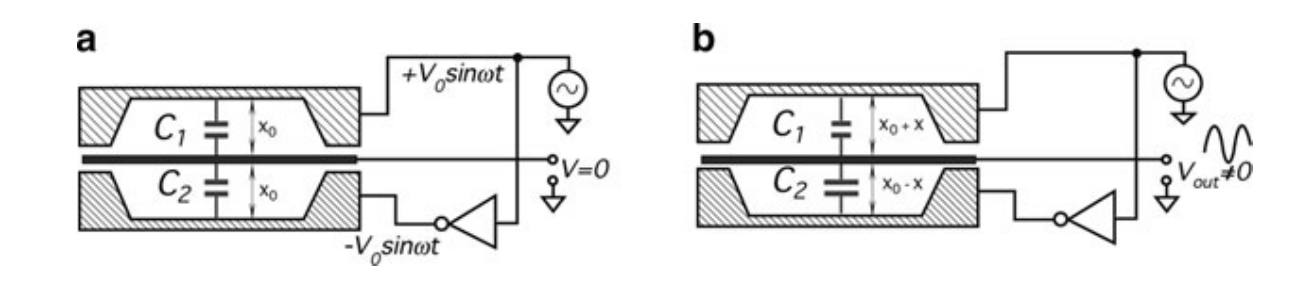
\includegraphics[width=\textwidth]{/LR/capacitive_sensors.png}
    \caption{Principle of operation for a flat-plate capacitive sensor. Adapted from \cite[Fig. 7.6]{handbook_sensors}.}
    \label{fig:capacitive_sensors}
\end{figure}

Capacitive sensors can be monopolar, differential (utilizing two capacitors), or a capacitive bridge can be utilized (using four capacitors) \cite{handbook_sensors}.
A typical capacitive pressure sensor is differential, with a diaphragm surface serving as the central plate, as depicted in Fig. \ref*{fig:capacitive_sensors}, creating a dual variable capacitor \cite{pressure_sens_calibration_stat_dyn}.
The capacitance changes when a load is applied to the diaphragm surface. 

Capacitive pressure sensors have broad measurement range, high sensitivity, accuracy and reliability, absence of contamination risk, large range of working temperatures (-70 \textdegree C to 400 \textdegree C).
The sensors are low-cost, highly sensitive devices mostly used in exceptional circumstances, such as miniature or even MEMS force sensors \cite*{multi_axis_force_sensors_review} and harsh environmental conditions.


\subsection{Electrical Resistance Strain Gauge}
The principle behind Electrical Resistance Strain Gauges (ERSGs) is the change in resistance caused 
by deformation, as explained in a study by official representative of Keller AG manufacturer \cite{keller_article}. 
Stretching or compressing of the piezoresistive material results in a change in the electric resistance of the sensor 
\cite{multi_axis_force_sensors_review}. 
% When the piezoresistive material is stretched or compressed, 
% it results in a change in the electric resistance of the sensor 
% \cite{multi_axis_force_sensors_review}. 
In order to accurately measure small changes in geometry, 
strain-gauge sensors are typically connected to a Wheatstone bridge.

Since the creation of the multi-axis force sensor in the 1970s, 
the strain-resistive pressure sensor has remained a classic measuring device \cite{3d_FBG_sensor}. 
However, these solutions tend to be expensive and require additional surface treatment of the substrate, 
as well as high-quality technology for bonding with a strain-resistant component 
\cite{my_love_pressure_photosensor, fingertip_based_FBG}. Load cells, which utilize strain gauges, 
face challenges in signal processing. These challenges include sensitivity to temperature and magnetic noise, 
the need for regular calibration, and difficulties in maintenance after the substrate undergoes plastic deformation.
% TODO: rephrase
Regarding response times, typical values of this measuring principle range from 1 to 10 ms. \cite{pressure_sens_calibration_stat_dyn}

\subsection{Fiber Bragg grating}
Fiber Bragg gratings (FBG) are the most popular optical pressure measurement methods. The FBG sensor is a specific type 
of distributed Bragg reflector that is created within a short section of optical fiber. 
Its function is to selectively reflect certain wavelengths of light while allowing all other wavelengths to pass through. 
When subjected to strain or temperature variations, the reflected wavelengths of an FBG shift accordingly. 
The magnitude of this wavelength shift is directly proportional to the applied load.
Several scientific papers, including Xiong L. et al. \cite{3d_FBG_sensor} and Guo Yu \cite{fingertip_based_FBG}, 
have documented the development of six-axis force sensors utilizing a fiber Bragg lattice. 
This design offers several advantages over strain-resistant sensors, such as immunity to electromagnetic interference, 
a compact profile, and lightweight construction. However, important to note that FBG-based sensors 
necessitate significant investments in optical signal demodulation equipment \cite{3d_FBG_sensor}, 
as well as surface treatment processes.

\subsection{Photointerrupter cell with barrier}

The optocoupler pressure sensor comprises three main components: a light emitter, two light receivers, and an interrupter positioned between emitter and one of the receivers \cite{my_love_pressure_photosensor}. 
When a load is applied to the sensor, the interrupter plate shifts, thereby altering the rate of light intensity on the measuring diode \cite{1990_optic}.
The signal from the second receiver is a reference and enables the cancellation of the optocoupler characteristics change, that effects whole system equally, caused by temperature, dirt and etc.

In the mathematical model of this type of cell, the barrier can be considered as a spring, making the applied force proportional to the deformation of the barrier.

This type of sensor has negligible hysteresis and repeatability error, since the vane movement amplitude to close the measuring diode is very small \cite*{pressure_sens_calibration_stat_dyn}.
Additionally, it offers a compact geometry and is cost-effective. % Moreover, since the optical surface usually is 

Compared to ERSG sensors, the photointerrupter measurement cell is less susceptible to electrical interference \cite*{my_love_pressure_photosensor}. 

The properties associated with hysteresis and the sensor's nominal range are primarily influenced by the type of barrier utilized \cite{my_love_pressure_photosensor}.
\begin{figure}[t]
\centering
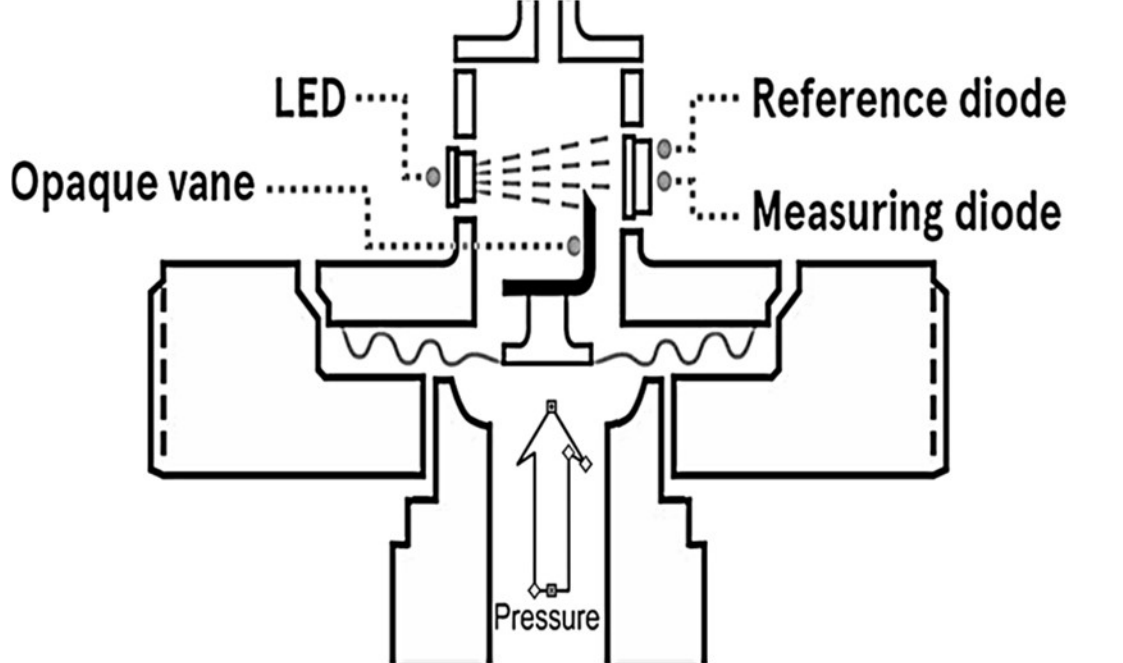
\includegraphics[width=0.5\textwidth]{optical_force_sensor.png}
\caption{Example of an optical pressure sensor. Adapted from \cite[Fig. 5]{pressure_sens_calibration_stat_dyn}.}
\label{fig:optical_sensor_arrangement}

\end{figure}

Other advantages of this type of pressure sensor, particularly important in certain industrial applications, include its long transmission distance and low chemical reactivity, making it ideal for operation in explosive-risk environments and intrinsically safe. 
The sensors using this measuring principle have a response time of about 100 $\mu$s and an average force resolution of 0.1 N over a 200 N measurement range \cite{pressure_sens_calibration_stat_dyn}.

% TODO: continue
The described characteristics of force sensor types force me to use the one in the research and try to apply the measurement principle in cells of my multi-axial force sensor.

\section{Metrics}
stiffness, nominal values, isotropy
In a coupled sensor an axis force component produces signal in more then one measurement cell, therefore calibration becomes more complicated.
% isotropy - какой контекст
%  взять характеристики датчика из учебника, которые подходят. Прочитать раздел с датчиками силы.
\subsection{Hysteresis}
% Add hysteresis graphs.  взять из учебника.
In certain systems, the sensor output varies based on the direction of load application. 
The difference between the outputs is referred to as hysteresis error \cite{handbook_sensors}, which represents the memory of the system.

\begin{figure}[t]
    \centering
    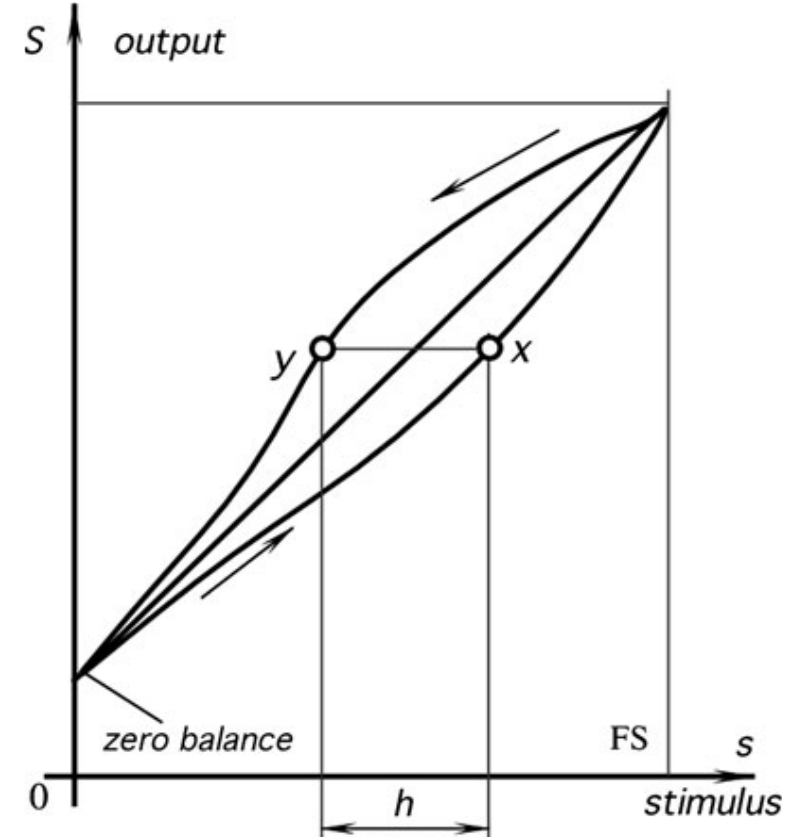
\includegraphics[width=0.5\textwidth]{/LR/hysteresis.png}
    \caption{Diagram illustrating the relationship between stimulus and signal in a system with hysteresis. Adapted from \cite[Fig. 2.11]{handbook_sensors}.}
    \label{fig:hysteresis}
\end{figure}    

\subsection{Coupling}
\label{lr_coupling}

One of the main metrics for multi-axial force sensor is degree of coupling, which determines the complexity of calibration matrix of a sensor 
\cite{decoupling_sliding_structure,multi_axis_force_sensors_review,CHAO1997105}. 
Dimensions coupling problem is one of the most common problems for multi-axial force sensors \cite{NN_decoupling}.
The degree of coupling among the axes directly impacts the accuracy of the sensor and the complexity of calibration 
\cite{decoupling_sliding_structure, multi_axis_force_sensors_review, CHAO1997105}. 
In a coupled sensor, an axis force component can produce signals in more than one measurement cell, 
thereby complicating the calibration process. However, designing and manufacturing highly decoupled structures can be challenging 
\cite{shape_optimization_decoupled}.

To reduce axis dependence one may change structure of the sensor or perform high precision calibration. 
Existing solutions for multi-axial force sensor structures are presented in the \ref{lr_constructions} section.

\section{Calibration}
\label{lr_calibration}
The multi-axis calibration has static and dynamic methods based on the applied force/pressure \cite{Static_Dynamic_Calibration_FlexiForce, pressure_sens_calibration_stat_dyn}.
A load usually is said to be static, if it remains constant during the measurement process. Accordingly, a load is said to be dynamic if it varies significantly in a short amount of time, usually, several times during the measurement.
The dynamic calibration is applied to sensors designed for highly dynamic environment with pressure pulsations or to determine the sensor response time \cite{pressure_sens_calibration_stat_dyn}. 
In my research the static calibration is sufficient, therefore, lets focus on the methods used in the multi-axis force sensors development.

Two static calibration methods exists: traditional and neural-networks based \cite{NN_decoupling, Deep_Learning_Calib}. % the first one writes about decoupling aka calibration - dummy article btw

Traditional method involves linear transformation (LT) of pressure cells output to the force and torque space using least-square-method (LSM) \cite{Deep_Learning_Calib}.
The mapping is represented with $N\times6$ matrix, where $N$ - number of uniaxial pressure sensors of the system \cite{Deep_Learning_Calib}.
The method defines two limitations \cite{Deep_Learning_Calib}:

\begin{itemize}
    \item The LT defines the linear dependency of sensor' output to the elastic body transformation.
    \item Matrix mapping representation requires load axes independence. 
\end{itemize}

% Нагнетание датчика мб надо добавить
In other words, the sensor output has to be linear to applied load with fully decoupled axes. 
The conditions are hard to satisfy, therefore many researches about structural sensors decoupling exists \cite{beam_structure_math,decoupling_sliding_structure,shape_optimization_decoupled,modal_sensor}.

Neural-networks based 

\dots

\subsection{How the ISO standart determines the calibration process}

— All force and moment channels are measured during the calibration process of each axis. All channels
are to be offset corrected in unloaded condition prior to the calibration test.

For force loading the force is applied within the neutral axes of the load cell.

In order to keep accuracy and to prevent  misalignment it should be avoided to exert torque within the mounting plane between load cell and fixture. This load case should be last in the sequence. It can cause rotation of the load cell within the fixture. Thus subsequently exerted loads can be shifted from the intended load axis

\subsubsection{misalignment determination}

For a loading in discrete steps or a continuous loading procedure, the output voltages in [mV/V] of all
transverse channels need to be recorded.
After the calibration of all axes, the current sensitivities of these channels are known and can be used
for the calculation of the crosstalk as percentage of the transducer axis’ calibration range.
For the force and moment channels, the transverse channels’ output voltage recorded in [mV/V]
(see NOTE 1) shall be converted to the physical dimension force or moment by applying the current
sensitivity determined from the calibration test before. 


\section{Constructions}
\label{lr_constructions}

Typically, the assessment of forces and moments in various directions is achieved by utilizing multiple strain-sensitive sensors affixed to a 
flexible substrate \cite{multi_axis_force_sensors_review}. The structure of a sensor plays a crucial role in its design as it governs 
characteristics such as stiffness, nominal values, isotropy, and the coupling among the measured axes 
\cite*{multi_axis_force_sensors_review,beam_structure_math}. 

To create optimized decoupled structures, engineers employ finite element analysis (FEM) 
\cite*{1990_optic, multi_axis_force_sensors_review, beam_structure_math}.

% Typically, the assessment of forces and moments in various directions is carried out through the 
% utilization of multiple strain-sensitive sensors that are affixed to a flexible substrate\cite{multi_axis_force_sensors_review}.
% The structure of a sensor is an essential component of its design, as governs characteristics such as stiffness, nominal values, isotropy, and the coupling among 
% the measured axes \cite*{multi_axis_force_sensors_review,beam_structure_math}. The last one determines the accuracy of the sensor and calibration complexity \cite{decoupling_sliding_structure,multi_axis_force_sensors_review,CHAO1997105}. 
% In a coupled sensor an axis force component produces signal in more then one measurement cell, therefore calibration becomes more complicated. 
% Nevertheless, the high-decoupled structures are hard to design and manufacture \cite{shape_optimization_decoupled}. 
% To create optimized decoupled structure engineers use finite element analysis (FEM) \cite*{1990_optic,multi_axis_force_sensors_review,beam_structure_math} 
% and with computational power growth creation of mechanically decoupled solutions becomes easier. 
% In their study Mayetin and Kucuk \cite{modal_sensor} created a modal sensor with average average interference error <3\%. The approach allows to replace failed structural elements.

% A multi-axis force sensor with a high coupling level 
% The configuration determines strain distribution and the position of the sensors \cite{beam_structure_math}. 
% In the multi-axis force sensors review \cite{multi_axis_force_sensors_review} authors proposed categorization for elastic structure designs.
% The types of six DOF force sensors structures: six DOF cross-beam, column-type, beam-column type, Stewart platform. Brief descriptions of each beam structure are in the next subsections.

% \subsection{Six DOF cross-beam structure}

\begin{enumerate}
    \item Rigid jointed cross-beams
\end{enumerate}
The most prevalent type of sensors used are rigid-joined sensors, primarily due to their solid beam structure, 
which facilitates simplified manufacturing. 
According to studies conducted by \cite{multi_axis_force_sensors_review, beam_structure_math}, 
rigid-joined cross beams exhibit reduced measurement isotropy and an increased level of coupling. 
The high level of coupling of rigid-joined sensors pushed researchers to find mechanically decoupled solutions.
A comprehensive compilation of rigid-joined cross-beam sensors can be found in \cite{multi_axis_force_sensors_review}.

\begin{enumerate}[resume]
    \item Flexible jointed cross-beams
\end{enumerate}

% TODO: Add reference to the figure flexible_beams
The flexible jointed structure was created to avoid the calibration complexity of mechanically coupled sensors \cite{shape_optimization_decoupled}. 
Want is a flexible joint of the cross-beam? Some researches define the flexible joint as a thin regions in the beam structure. 
Those regions are elastic compared to the whole beam, therefore they act as a damper and reduce the cross dimension coupling. 

The second type of flexible jointed cross-beams is the $WHICH_WORD_TO_USE$. Their constructions has additional mechanical component as joint, for example, bearings or hinges.

\begin{figure}[H]
    \begin{subfigure}[b]{0.3\textwidth}
        \label{fig:flexible_beams_a}
        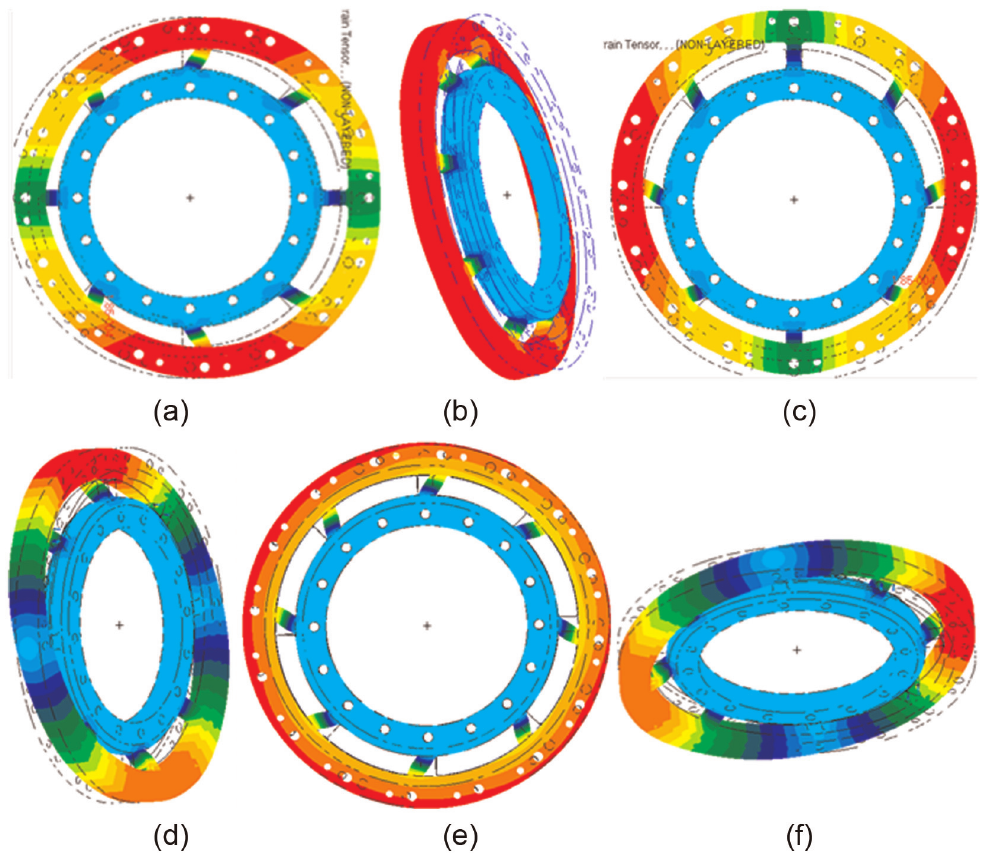
\includegraphics[width=\textwidth]{flexible_beam.png}
        \caption*{thin joints}
    \end{subfigure}
    \begin{subfigure}[b]{0.3\textwidth}
        \label{fig:flexible_beams_b}
        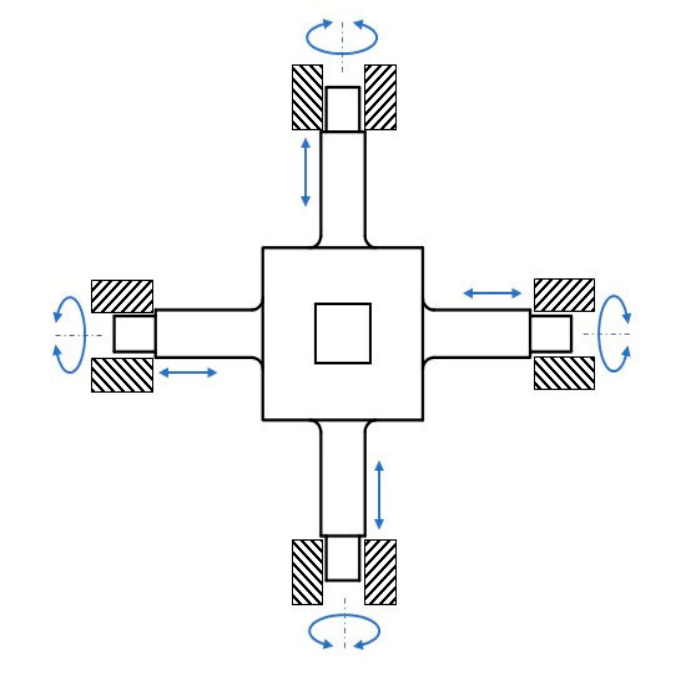
\includegraphics[width=\textwidth]{sliding_beam.png}
        \caption*{sliding joints}
    \end{subfigure}
    \caption{Example of flexible joined beams structures for multi-axial sensors.}
    \label{fig:flexible_beams}
\end{figure}

\begin{enumerate}[resume]
    \item Modal cross-beams
\end{enumerate}

With the advancement in computational power, the creation of mechanically decoupled solutions has become more accessible. 
In their study, Mayetin and Kucuk \cite{modal_sensor} developed a modal sensor with an average interference error of less than 3\%.
This approach allows for the replacement of failed structural elements, enhancing the overall reliability and longevity of the sensor.
\begin{figure}[H]
    \label{fig:modal_sensor}
    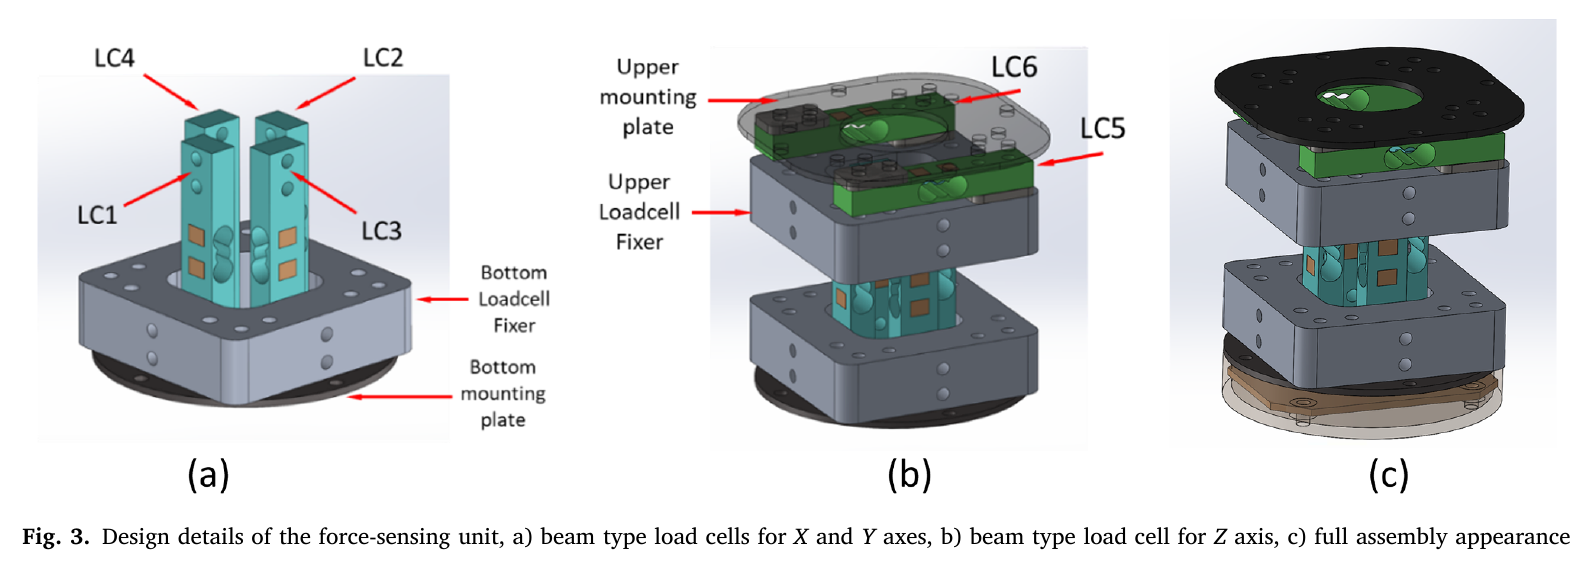
\includegraphics[width=\textwidth]{modal_sensor.png}
    \caption*{modal sensor from \cite{modal_sensor}}
\end{figure}

% \begin{enumerate}[resume]
%     \item Dual-layer cross-beams
% \end{enumerate} 

% Перед констракшеном

\section{Conclusion}
\label{lr_conclusion}
In this literature review, we have explored the research conducted by Hosseinabadi and Salcudean \cite{perfect_sensor} and the model proposed by
 \cite{my_love_pressure_photosensor} for a mechanically decoupled six DOF force sensor with low cross-coupling error and high resolution to scale 
 ratio of 0.0001\%. 
 Additionally, we have examined the 3-DOF force sensor structure proposed in \cite{modal_sensor}, 
 which features four independent beams with an average interference error of less than \( 3 \% \).

Building upon these previous studies, the current research aims to develop a mechanically decoupled modal structure for a six DOF force sensor,
utilizing the measurement cell invented by \cite*{my_love_pressure_photosensor}. 
The focus of this study will be on calculating the cross-coupling interference, resolution to scale ratio, and hysteresis of the sensor. 

% \cite*{optic_mirror}
% This enables the development of a versatile solution suitable for a wide range of loads. The design offers several benefits, including protection against electromagnetic interference, the ability to adjust the range of values by modifying the barrier, and cost-effectiveness and availability of the structural elements.